\documentclass[12pt]{article}
\usepackage[spanish,mexico]{babel}
\usepackage[utf8]{inputenc}
\usepackage{times}
\usepackage{physics,amsmath,amssymb,siunitx,codehigh,cancel,float}
\usepackage{hyperref}
\usepackage{csquotes,ragged2e}
\usepackage{tabularray}
\UseTblrLibrary{booktabs}
\usepackage{tablefootnote}
\usepackage{graphicx}
\usepackage{booktabs,minted}
\usepackage{array}
\usepackage{ragged2e}
\usepackage{pgffor}  
\usepackage[table,xcdraw,x11names]{xcolor}
\usepackage{geometry}
\usepackage{setspace}
\geometry{a4paper, margin=1in}
\usepackage{soul}
\usepackage{lscape}
\title{Entregable Preliminar}
\date{\today}
\author{Jocelyn Janet Parés Ramos & 
        Juan Pablo de la Vega Lozano &
        Carlos Alberto Torre Sánchez &
        Ana Camila Murillo Fernández &
        Gael García Zúñiga}

\begin{document}

\maketitle
\newpage


\section{Resumen}
En este trabajo analizamos el comportamiento de una cortadora rotativa de césped para la empresa John Deere. Nuestro enfoque principal fue diseñar un modelo que simule el movimiento tanto del disco como de las cuchillas, con el fin de estudiar qué factores afectan su desempeño y qué aspectos se pueden mejorar. El modelo considera las ecuaciones que gobiernan el movimiento circular del sistema, buscando una representación realista de la dinámica involucrada.Para resolver el sistema de ecuaciones diferenciales de segundo orden, implementamos el método de Runge-Kutta 4(5). Se definieron múltiples parámetros clave como el torque del motor, la fricción viscosa y los ángulos iniciales, lo cual nos permitió observar cómo responde el sistema ante distintos escenarios.Las conclusiones más relevantes del trabajo son que este modelo nos muestra claramente el valor hacia el cual la velocidad angular se estabiliza, permitiendo anticipar el rendimiento del sistema con distintos motores o condiciones de operación. 

\section{Introducción}
La eficiencia energética de la maquinaria, en cualquier sector, es clave para reducir costos y optimizar tiempos de operación. En este reporte analizaremos las cortadoras rotativas de césped John Deere, especificamente el modelo HX10, a partir de un modelo mecánico que describe el comportamiento de sus cuchillas bajo densidades de pasto variables. La dinámica de estas cuchillas, montadas en un disco giratorio, implica acoplamientos cinemáticos y de momento de inercia que exigen un tratamiento numérico preciso para capturar tanto los transitorios como las oscilaciones amortiguadas. Para ello, empleamos métodos espectrales y numéricos, en particular integradores de paso variable como \texttt{RK45}, que resultan eficaces para resolver sistemas acoplados de ecuaciones de segundo orden sin incurrir en elevados costos computacionales. Las ecuaciones que se utilizaron para modelar el movimiento de cada cuchilla son:
\begin{equation}
	\begin{aligned}
		\frac{1}{3} m L^2 \ddot{\theta}_1 &= \left( \frac{1}{2} m r L \dot{\phi}^2 \sin\theta_1 + \frac{1}{3} m L^2 \dot{\phi}^2 \sin\theta_1 \cos\theta_1 \right) - \left( \frac{1}{2} b_1 r L^2 \dot{\phi} \sin\theta_1 + \frac{1}{3} b_1 L^3 \dot{\theta}_1 \right), \\
		\frac{1}{3} m L^2 \ddot{\theta}_2 &= \left( \frac{1}{2} m r L \dot{\phi}^2 \sin\theta_2 + \frac{1}{3} m L^2 \dot{\phi}^2 \sin\theta_2 \cos\theta_2 \right) - \left( \frac{1}{2} b_2 r L^2 \dot{\phi} \sin\theta_2 + \frac{1}{3} b_2 L^3 \dot{\theta}_2 \right)
        \end{aligned}
	\end{equation}
    
	Y para el movimiento del disco:

	\begin{equation} (\frac{1}{2}MR^2 + \frac{2}{3}mL^2)\ddot{\phi} = \tau_{\text{motor}}(t) - \sum_{i=1}^{2} [b_i \dot{\phi} \sin{\theta_i} \left(\frac{rL^2}{2} + \frac{L^3\cos{\theta_i}}{3}\right) + \frac{1}{3}b_i L^3 \dot{\theta}_i \sin{\theta_i}] \end{equation}
	

\section{Metodología}

Se ha desarrollado un modelo matemático y computacional para simular el comportamiento dinámico del sistema de corte rotatorio. El sistema consiste en un disco central al que se acoplan dos cuchillas en los extremos, las cuales interactúan con pasto durante su movimiento. 

\begin{figure}[H]
    \centering
    \begin{minipage}[b]{0.4\textwidth}
    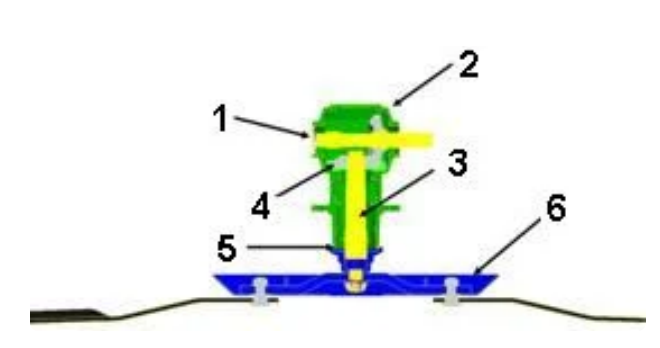
\includegraphics[width=\textwidth]{Blades.png}
  \end{minipage}
  \hfill
  \begin{minipage}[b]{0.4\textwidth}
    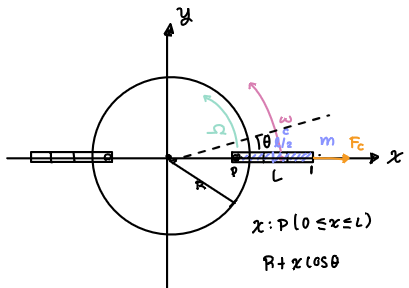
\includegraphics[width=\textwidth]{diagrama.png}
  \end{minipage}
    \caption{Diagrama de las cuchillas}
    \label{fig:enter-label}
\end{figure}

Dado esto, se creó un código de Python para posteriormente obtener simulaciones del sistema. Las variables son las siguientes: 

\begin{itemize}
    \item \textbf{un disco de radio $R$:} 0.536 m
    \item \textbf{una masa $M$ del disco:} 40.38 kg  
    \item \textbf{un ángulo de rotación $\phi(t)$ del eje central del disco:} 0-2$\pi$ rad
    \item \textbf{dos cuchillas de longitud $L$:} 0.54 m
    \item \textbf{una masa $m$ de las cuchillas:} 5.33 kg
    \item \textbf{los pivotes de las cuchillas a una distancia radial $r$:} 0.413 m
    \item \textbf{un ángulo relativo de oscilación $\theta_i(t)$, con $i = 1, 2$:} 0-2$\pi$ rad
\end{itemize}

\subsection{Modelo analítico}
El sistema se encuentra en un plano horizontal sin fricción con el suelo. Se considera fricción viscosa tanto en el eje del disco como en los pivotes de las cuchillas. La resistencia del pasto se modela como una fricción distribuida espacialmente, dependiente de la posición $(x, y)$ de las puntas de las cuchillas y se utiliza un torque constante $\tau_{motor}(t) = 2300$ Nm aplicado al disco.

Para las fuerzas se consideran las siguientes contribuciones de torque:

\subsubsection{Torque por Fuerzas Centrífugas en las Cuchillas}
Cada segmento diferencial de masa de una cuchilla sufre una aceleración centrífuga $a = (r + x \cos \theta) \dot{\phi}^2$, generando un torque de:

$$
\tau_{centr, i} = \frac{1}{2}mrL \dot{\phi}^2 \sin \theta_i + \frac{1}{3}mL^2 \dot{\phi}^2 \sin \theta_i \cos \theta_i.
$$

\subsubsection{Torque Viscoso del Pasto (Fricción)}
El torque de resistencia debida al pasto sobre cada cuchilla considera dos componentes:

 Por rotación del disco:
  $\tau_{pasto,d,i} = b_i \dot{\phi} \sin \theta_i (r L^2 / 2)$
Por rotación de la cuchilla:
  $\tau_{pasto,th,i} = b_i \dot{\theta}_i \sin \theta_i (L^3 / 3)$

Se define $b_i$ como un coeficiente local que depende de la posición de la punta de cada cuchilla en el campo espacial interpolado de densidad de pasto $\rho(x, y)$.

\subsubsection{Torque Total sobre el Disco}
El torque total que actúa sobre el disco se expresa como:

$$
I_{tot} \ddot{\phi} = \tau_{motor} - \sum_{i=1}^{2} (\tau_{pasto,di} + \tau_{pasto,th,i}) - c_{disk} \dot{\phi},
$$

donde $I_{tot} = I_{disco} + 2(I_{cuchilla} + m r^2)$, y $c_{disco}$ representa el coeficiente de amortiguamiento del disco.

\subsubsection{Sistema de Ecuaciones Diferenciales}
El sistema completo consiste en 6 variables dinámicas: $\phi, \dot{\phi}, \theta_1, \dot{\theta}_1, \theta_2, \dot{\theta}_2$. Se formula un sistema de ecuaciones diferenciales ordinarias (EDOs) de segundo orden, el cual se integra numéricamente utilizando \texttt{solve\_ivp} del paquete \textit{SciPy}

\subsubsection{Campo de Densidades de Pasto ($b(x,y)$)}
Para capturar la variabilidad espacial de la resistencia del pasto se define una malla cartesiana sobre el plano $(x, y)$ del disco. Se usa una función de densidad arbitraria, en este caso se optó pot usar$\rho(x, y) = 1 + 0.5 \sin\left(\frac{2\pi X}{R}\right) \cos\left(\frac{2\pi Y}{R}\right)$, no obstante se puede definir cualquier función de densidad. Se utiliza \texttt{RegularGridInterpolator} para interpolar valores de $\rho$ en coordenadas arbitrarias, y obtener el valor local de $b$ en cada instante de tiempo según la posición de la punta de cada cuchilla.

\subsection{ Simulación Computacional}
Se usó Python con las bibliotecas \texttt{NumPy}, \texttt{SciPy} y \texttt{Matplotlib}. Se definieron condiciones iniciales: $\phi(0) = 0$, $\dot{\phi}(0) = 0$, $\theta_1(0) = 0.1$, $\theta_2(0) = 1.0$, $\dot{\theta}_1(0) = \dot{\theta}_2(0) = 0$. El intervalo de simulación fue $t \in [0, 50]$ s. El código es el siguiente:

\begin{minted}[fontsize=\footnotesize]{python}
import numpy as np
import matplotlib.pyplot as plt
from scipy.integrate import solve_ivp
from scipy.interpolate import RegularGridInterpolator

# -- Parámetros del sistema --
M = 40.38      # masa del disco
m = 5.33       # masa de cada cuchilla
R = 0.536     # radio del disco
r = 0.413       # distancia pivote
L = 0.54     # longitud de la cuchilla

# Coeficientes base
b1 = b2= 0.01     # coeficiente base cuchilla 1
c_disk = 1   # fricción viscosa del disco
c_th1 = c_th2 =9    # amortiguamiento pivote cuchilla 1

theta01 = 0.1  # ángulo inicial cuchilla 1
theta02 = 1        # ángulo inicial cuchilla 2

# Función de torque del motor
def tau_motor(t):
    return 2300

# Momentos de inercia
I_disc  = 0.5 * M * R**2
I_blade = (1/3) * m * L**2

# Campo de densidad de pasto
x_grid = np.linspace(-R, R, 200)
y_grid = np.linspace(-R, R, 200)
X, Y  = np.meshgrid(x_grid, y_grid)
rho   = 1 + 0.5 * np.sin(2 * np.pi * X / R) * np.cos(2 * np.pi * Y / R)
interpolator = RegularGridInterpolator((x_grid, y_grid), rho,
                                       bounds_error=False, fill_value=1.0)

def b_field(x_tip, y_tip, base_b):
    return base_b * interpolator((x_tip, y_tip))

# Definición de torques

def tau_disc_b(phi_dot, theta, theta_dot, b):
    term_phi  = b * phi_dot   * np.sin(theta) * (r*L**2/2 + (L**3/3)*np.cos(theta))
    term_th   = b * theta_dot * np.sin(theta) * (L**3/3)
    return term_phi + term_th


def tau_blade_b(phi_dot, theta, theta_dot, b):
    term_cut  = b * phi_dot   * np.sin(theta) * (r*L**2/2)
    term_drag = b * theta_dot * np.sin(theta) * (L**3/3)
    return term_cut + term_drag


def theta_dd(phi_dot, theta, theta_dot, b, c_th):
    cent1 = 0.5 * m * r * L * phi_dot**2 * np.sin(theta)
    cent2 = (1/3) * m * L**2 * phi_dot**2 * np.sin(theta) * np.cos(theta)
    tau_g = tau_blade_b(phi_dot, theta, theta_dot, b)
    tau_d = -c_th * theta_dot
    return (-cent1 - cent2 - tau_g + tau_d) / I_blade

# Sistema de ecuaciones
def odes(t, y):
    phi, phidot, th1, dth1, th2, dth2 = y
    I_tot = I_disc + 2*(m*r**2 + I_blade)

    # Posiciones pivote y puntas
    x_piv = r * np.cos(phi)
    y_piv = r * np.sin(phi)
    x_tip1 = x_piv + L * np.cos(phi + th1)
    y_tip1 = y_piv + L * np.sin(phi + th1)
    x_tip2 = x_piv + L * np.cos(phi + th2)
    y_tip2 = y_piv + L * np.sin(phi + th2)

    # Coeficientes locales
    b1_loc = b_field(x_tip1, y_tip1, b1)
    b2_loc = b_field(x_tip2, y_tip2, b2)

    # Torques de pasto sobre el disco
    t1 = tau_disc_b(phidot, th1, dth1, b1_loc)
    t2 = tau_disc_b(phidot, th2, dth2, b2_loc)

    # Ecuación del disco
    phidd = (tau_motor(t) - t1 - t2 - c_disk*phidot) / I_tot

    # Aceleraciones de las cuchillas
    dth1dd = theta_dd(phidot, th1, dth1, b1_loc, c_th1)
    dth2dd = theta_dd(phidot, th2, dth2, b2_loc, c_th2)

    return [phidot, phidd, dth1, dth1dd, dth2, dth2dd]

# Condiciones iniciales y resolución
y0 = [0, 0, theta01, 0, theta02, 0]
t_span = (0, 50)
sol = solve_ivp(odes, t_span, y0, method='RK45',
                rtol=1e-2, atol=1e-5, max_step=0.5)

# Extracción de resultados
t = sol.t
phi      = sol.y[0]
phi_dot  = sol.y[1]
theta1   = sol.y[2]
dth1     = sol.y[3]
theta2   = sol.y[4]
dth2     = sol.y[5]

# Coordenadas disco y puntas
x_disk = R * np.cos(phi)
y_disk = R * np.sin(phi)
x_piv  = r * np.cos(phi)
y_piv  = r * np.sin(phi)
x_tip1 = x_piv + L * np.cos(phi + theta1)
y_tip1 = y_piv + L * np.sin(phi + theta1)
x_tip2 = x_piv + L * np.cos(phi + theta2)
y_tip2 = y_piv + L * np.sin(phi + theta2)
\end{minted}

El marco de simulación propuesto es replicable y puede servir como base para optimizar parámetros de diseño o evaluar estrategias de control del sistema de corte. 

\section{Resultados}
Al momento de correr el código, fue claro que el sistema programado era altamente propenso a dar resultados impredecibles e incomprensibles. Observamos que los resultados también variaban mucho dependiendo de los coeficientes base. Es por esta razón que experimentamos con los coeficientes hasta encontrar resultados que daban más sentido.\\

Después de encontrar parámetros que daban los resultados esperados, obtuvimos las siguientes gráficas para el disco:


\begin{figure}[H]
    \centering
    \begin{minipage}[b]{0.3\textwidth}
    \includegraphics[width=\textwidth]{Imagen2.png}
  \end{minipage}
  \hfill
  \begin{minipage}[b]{0.3\textwidth}
    \includegraphics[width=\textwidth]{Imagen1.png}
  \end{minipage}
  \hfill
  \begin{minipage}[b]{0.3\textwidth}
    \includegraphics[width=\textwidth]{Imagen3.png}
  \end{minipage}
    \caption{Gráficas obtenidas del angulo del disco con respecto al tiempo, la trayectoria circular del disco y la velocidad angular, respectivamente.}
    \label{fig:enter-label}
\end{figure}

 En la primera figura, observamos el ángulo del disco con respecto al tiempo. Con esta información podemos concluir que el movimiento del disco tiene sentido; estamos midiendo su posición angular, así que por cada $2\pi$ valores hay una rotación. De esto podríamos conseguir el número de rotaciones en cierto tiempo, lo cual es un dato importante para las personas que utilizan este tipo de tecnologías. \\

 
En la segunda imagen, se observa la trayectoria espacial del disco. Esta gráfica sirve más para corroborar que los resultados tengan sentido, y esta se ha mantenido consistente a lo largo de toda la experimentación con los valores, únicamente variando cuando reducimos el torque total de tal manera que no logra cubrir toda la trayectoria circular.\\

La 3era gráfica demuestra la velocidad angular del disco con respecto al tiempo;se observa que conforme más tiempo pasa, la tasa de crecimiento se reduce. Después de correr la simulación por más tiempo, se observa que esta velocidad se aproxima al valor del torque del motor. El único dato que modifica esta asíntota es el coeficiente de fricción viscosa del disco: mientras más grande es, la asíntota baja a un valor menor.\\


	Por otro lado, obtuvimos representaciones visuales del movimiento de las cuchillas. En este caso, el sistema que estamos graficando es el ángulo de la cuchilla con respecto a la normal del disco. En otras palabras, si la cuchilla esta perfectamente extendida, el ángulo sería 0. Agregamos un ángulo inicial de 0.1, para que no tome mucho tiempo en estabilizarse el sistema. Aquí podemos observar las gráficas obtenidas:

        
\begin{figure}[H]
    \centering
    \begin{minipage}[b]{0.3\textwidth}
    \includegraphics[width=\textwidth]{Imagen4.png}
  \end{minipage}
  \hfill
  \begin{minipage}[b]{0.3\textwidth}
    \includegraphics[width=\textwidth]{Imagen5.png}
  \end{minipage}
  \hfill
  \begin{minipage}[b]{0.3\textwidth}
    \includegraphics[width=\textwidth]{Imagen6.png}
  \end{minipage}
    \caption{Gráficas obtenidas del ángulo de la cuchilla con respecto al tiempo, la trayectoria de la cuchilla y la velocidad angular, respectivamente.}
    \label{fig:enter-label}
\end{figure}

Primero, tenemos el ángulo de las cuchillas con respecto al tiempo. Se puede observar que la gráfica inicia en 0.1, lo cual se alinea con la condición inicial establecida. Después logra estabilizarse después de oscilar por muy poco tiempo. La magnitud de la fuerza centrífuga del sistema hace que se estabilice en mayor o menor tiempo.\\

	Por otro lado, está la trayectoria de la cuchilla. De la misma manera que la trayectoria del disco, esta gráfica sirve para verificar que el sistema funcione correctamente. Podemos observar que se ve muy similar a la otra trayectoria, pero los límites de la gráfica son mayores. Esto tiene sentido, ya que la distancia de las cuchillas al centro es mayor que la del disco por su propia cuenta.\\
    
	Finalmente, tenemos la velocidad angular de la cuchilla con respecto al tiempo. En este caso, tenemos que la velocidad inicia en 0, pero al inicio varía mucho. Esto se debe a los cambios en posición que ocurren en el proceso de estabilización. El mismo momento que el ángulo llega a un estado estacionario, ocurre lo mismo en la velocidad, ya que a este punto no hay cambios significativos en la posición angular de la cuchilla, lo cual implica lo mismo de la velocidad.

\section{Discusión}
Durante la ejecución del código, notamos que el sistema es altamente sensible a los parámetros que se le asignan; se comporta de manera caótica ante pequeños cambios. Esto nos llevó a ajustar manualmente los coeficientes hasta obtener resultados físicamente coherentes.\\

Una forma de hacer este modelo más útil para la empresa sería desarrollar una interfaz sencilla, que permita explorar los resultados bajo distintos materiales, densidades de vegetación o parámetros geométricos. Esto facilitaría la toma de decisiones sin necesidad de conocimientos técnicos avanzados.\\

Sin embargo, nuestro modelo presenta algunas limitaciones. En simulaciones con parámetros grandes o condiciones extremas, el tiempo de cómputo se incrementa notablemente y los resultados pueden volverse difíciles de interpretar. Además, no se considera la interacción entre cuchillas ni la deformación del pasto. Aunque en nuestras pruebas esto no alteró de forma significativa las velocidades obtenidas, el modelo podría mejorarse integrando métodos numéricos más precisos o incorporando más variables físicas relevantes.


\section{Conclusión}
Este trabajo nos permitió simular el comportamiento de una cortadora rotativa, enfocándonos en el disco y las cuchillas bajo distintos parámetros. Una de las conclusiones más relevantes es que logramos obtener resultados consistentes con lo que se esperaría en un escenario real, lo que valida el modelo propuesto. También observamos que la velocidad angular del disco se estabiliza en un valor definido por el torque del motor y la fricción viscosa, lo cual es útil para ajustar el sistema a distintas condiciones de operación. En el caso de las cuchillas, el modelo mostró que se estabilizan rápidamente debido a la fuerza centrífuga, lo que tiene sentido físico.\\

Un punto importante es que el sistema es muy sensible a los valores de entrada. Pequeños cambios en los coeficientes pueden alterar mucho el resultado. Esto indica que, si se desea usar el modelo en la industria, sería útil desarrollar una herramienta que permita modificar estos parámetros fácilmente sin requerir conocimientos técnicos avanzados.
En general, el modelo es una buena base para seguir explorando mejoras en el diseño de cortadoras rotativas y puede ampliarse en el futuro para considerar más factores físicos y lograr una simulación más precisa.

\section{Referencias}

Cortadoras de Césped | John Deere MX. (n.d.). Retrieved 23 May 2025, from \url{https://www.deere.com.mx/es/cortadoras-de-c%C3%A9sped/}

John Deere Parts Lookup -HX10 Rotary Cutter Lift-Type \& Offset Versions are Shown. Pull-Type \& Semi-Mount Versions are also available. Manufactured (1999- ) -PC2792. (n.d.). Retrieved 23 May 2025, from \url{https://www.weingartz.com/illustrated-diagram/john-deere-parts-lookup/model-hx10-rotary-cutter-lift-type-offset-versions-are-shown-pull-type-semi-mount-versions-are-also-available-manufactured-1999-pc2792/4275-372}

solve\_ivp—SciPy v1.15.3 Manual. (n.d.). Retrieved 23 May 2025, from \url{https://docs.scipy.org/doc/scipy/reference/generated/scipy.integrate.solve_ivp.html}

Weiser, A., \& Zarantonello, S. E. (1988). A note on piecewise linear and multilinear table interpolation in many dimensions. Mathematics of Computation, 50(181), 189–196. \url{https://doi.org/10.1090/S0025-5718-1988-0917826-0}


\end{document}
